\documentclass{article}
\usepackage[utf8]{inputenc}
\usepackage{tkz-euclide}
\usepackage{graphicx}
\usepackage{hyperref}
\usepackage{amsmath}
\usepackage{amssymb}
\usepackage{tikz}
\usetkzobj{all}

\begin{document}

Convención del signo de los angulos

$\angle{QOP} > 0$
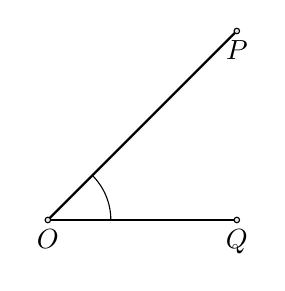
\begin{tikzpicture}[scale=.8]

% definitions
\tkzDefPoint(0,0){O}
\tkzDefPoint(3,3){P}
\tkzDefPoint(3,0){Q}
\tkzMarkAngle[label=QOP, size=1](Q,O,P)

\tkzDrawSegments[thick](O,P)
\tkzDrawSegments[thick](O,Q)
\tkzDrawPoints(O,P,Q)

% labels
\tkzLabelPoints(Q,O,P)
\end{tikzpicture}

$\angle{QOP} < 0$  o $\angle{QOP} > 12:00:00h $ (los angulos mayores de 180 grados se representan con valor negativo)
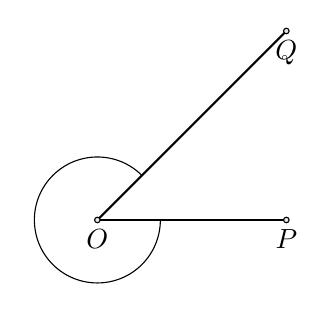
\begin{tikzpicture}[scale=.8]

% definitions
\tkzDefPoint(0,0){O}
\tkzDefPoint(3,3){Q}
\tkzDefPoint(3,0){P}
\tkzMarkAngle[label=QOP, size=1](Q,O,P)

\tkzDrawSegments[thick](O,P)
\tkzDrawSegments[thick](O,Q)
\tkzDrawPoints(O,P,Q)

% labels
\tkzLabelPoints(Q,O,P)
\end{tikzpicture}



\begin{itemize}
\item O: centro de la tierra y de la esfera celeste (esfera que contiene la esfera de la tierra, el plano ecuadorial terrestre se extiende al plano ecuadorial celeste y la comparte igual que la tierra en 2 hemisferios: norte y sur y el plano del meridiano 0 se puede extender para toda la esfera celeste). La correspondiente de la latitud en la tierra es la declinación para la esfera celeste (negativa si el objeto a observar está en hemisferio sur celeste) y para la longitud la declinación recta(positiva desde el meridiano 0 en el sentido de la rotación dela tierra en torno a su propio eje y negativa en el otro sentido)
\item P: punto del observador
\item T: posicion del objeto observado
\end{itemize}

Proyeccion longitudinal
P está en el hemisferio norte(latitud positiva) 
\vspace{5cm}


Declinacion negativa
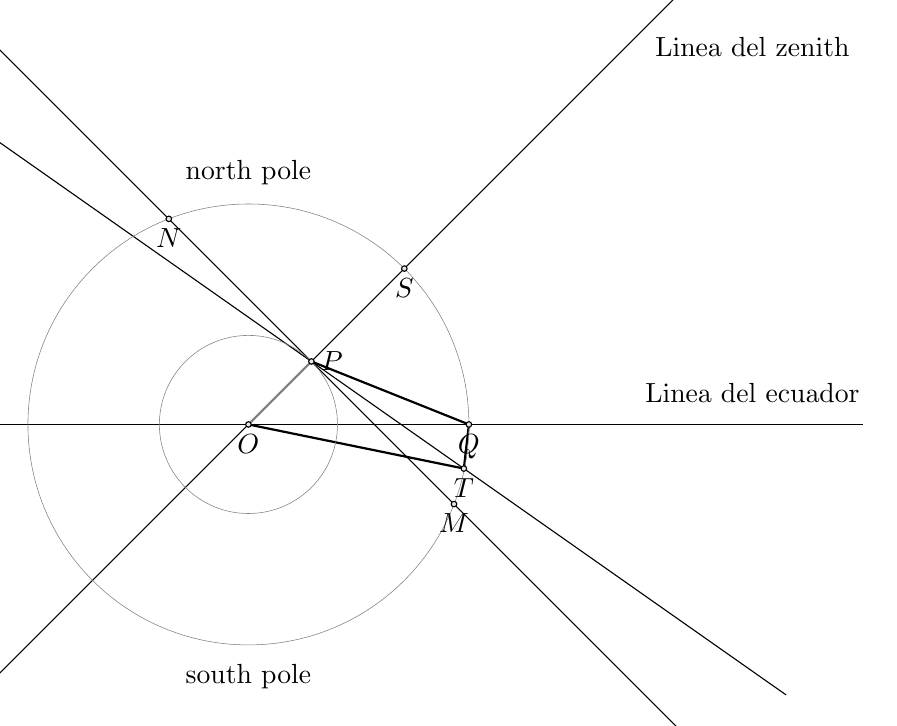
\begin{tikzpicture}[scale=.8]

% definitions
\tkzDefPoint(0,0){O}
\tkzDefPoint(1,1){P}
\tkzDefPoint(3.5,0){Q}
\tkzDefPoint(3.42,-0.7){T}

\tkzDefPointWith[orthogonal](P,O) \tkzGetPoint{P1} % find a point P1 orthogonal to PO
\tkzInterLC(P,P1)(O,Q) \tkzGetPoints{M}{N} % find intersections of a line passing through A and Q with the large circle 
\tkzInterLC(O,P)(O,Q) \tkzGetPoints{P4}{S} % find intersections of a line passing through A and Q with the large circle 
\draw [shorten >= -5cm, shorten <=-5cm] (P4)--(S);
\draw [shorten >= -5cm, shorten <=-5cm] (O)--(Q);
\node at (8,0.5){Linea del ecuador} ; 
\node at (8,6){Linea del zenith} ; 
\draw [shorten >= -5cm, shorten <=-5cm] (P)--(T) ;
\draw [shorten >= -5cm, shorten <=-5cm] (M)--(N) ;
%\tkzMarkAngle[label=lat, size=1](Q,O,P)

\tkzDrawSegments[thick](O,T)
\tkzDrawSegments[thick](T,Q)
\tkzDrawSegments[thick](P,Q)
%\tkzMarkAngle[](Q,O,T)
%\tkzMarkAngle[label=dec, size=1](Q,P,T)
%\tkzMarkAngle[label=zd, size=1](P4,P,T)
% drawing
\tkzDrawCircle(O,P)
\tkzDrawCircle(O,Q) 
\node at (0,4){north pole};
\node at (0,-4){south pole};
\tkzDrawSegments[thick,gray](O,P)
\tkzDrawPoints(O,P,Q,T,M,S,N)

% labels
\tkzLabelPoints(Q,T,O,M,S,N)
\tkzLabelPoints[right](P)
\end{tikzpicture}

\vspace{5cm}

Declinacion positiva
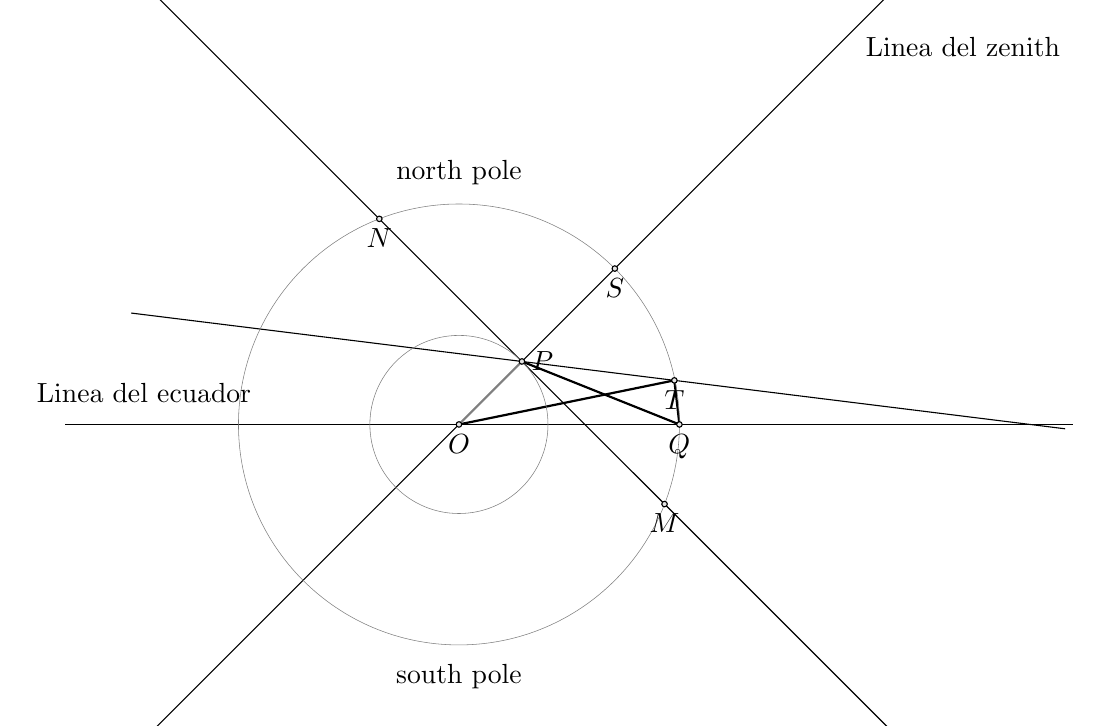
\begin{tikzpicture}[scale=.8]

% definitions
\tkzDefPoint(0,0){O}
\tkzDefPoint(1,1){P}
\tkzDefPoint(3.5,0){Q}
\tkzDefPoint(3.42,0.7){T}
\node at (-5,0.5){Linea del ecuador} ; 
\node at (8,6){Linea del zenith} ; 

\tkzDefPointWith[orthogonal](P,O) \tkzGetPoint{P1} % find a point P1 orthogonal to PO
\tkzInterLC(P,P1)(O,Q) \tkzGetPoints{M}{N} % find intersections of a line passing through A and Q with the large circle 
\tkzInterLC(O,P)(O,Q) \tkzGetPoints{P4}{S} % find intersections of a line passing through A and Q with the large circle 
\draw [shorten >= -5cm, shorten <=-5cm] (P4)--(S);
\draw [shorten >= -5cm, shorten <=-5cm] (O)--(Q) ;
\draw [shorten >= -5cm, shorten <=-5cm] (P)--(T) ;
\draw [shorten >= -5cm, shorten <=-5cm] (M)--(N) ;
%\tkzMarkAngle[label=lat, size=1](Q,O,P)

\tkzDrawSegments[thick](O,T)
\tkzDrawSegments[thick](T,Q)
\tkzDrawSegments[thick](P,Q)
%\tkzMarkAngle[](Q,O,T)
%\tkzMarkAngle[label=dec, size=1](Q,P,T)
%\tkzMarkAngle[label=zd, size=1](P4,P,T)
% drawing
\tkzDrawCircle(O,P)
\tkzDrawCircle(O,Q)
\node at (0,4){north pole};
\node at (0,-4){south pole};
\tkzDrawSegments[thick,gray](O,P)
\tkzDrawPoints(O,P,Q,T,M,S,N)

% labels
\tkzLabelPoints(Q,T,O,M,S,N)
\tkzLabelPoints[right](P)
\end{tikzpicture}


\vspace{5cm}
\begin{itemize}
\item OQ: linea del ecuador
\item OP: linea del zenit del observador(la linea que une el observador con el centro de la tierra) perpendicular en la linea del horizonte MN(solo se pueden ver objetos en el arco MSN: objetos con declinación entre -(90$^\circ$ - latitude) y 180$^\circ$ - (90$^\circ$ - latitude) )
\item PT: linea de vision del observador
\item $\angle{QPT}$ Para la proyeccion longitudinal es declinacion medida por el telescopio(negativa si la estrella está debajo del plano ecuadorial) - el angulo en el cielo entre la dirección del telescopio orientado hacia el objeto que observamos y la direccion del telescopio orientado hacía un objeto que está en el ecuador celeste. 
\item $\angle{QOT}$  declinacion  de la estrella (negativa si la estrella está debajo del plano ecuadorial) - medida desde un punto que esta en el ecuador de la tierra 
\item $\angle{QOP}$  latitud
\item $\angle{TPS}$  proyeccion en este plan del angulo zenith distance(formado por la linea del zenith y la direccion en cual apunta el telescopio) 
\item En práctica esta es zenith distance (el azimuth no cuenta) ZD medida en grados  (dd:mm:ss) con dd entre 00 y 90
y Airmass se aproxima como 1 / cos(ZD)


\end{itemize}
\begin{description}
\item $\angle{POQ} = \angle{POT} + \angle{TOQ}$
\item Q(el objeto de referrencia) está muy lejos asi que las distancias $OQ, PQ, PT, OT \gg OP$(el radio de la tierra) y  $\angle{TPQ}\approx \angle{TOQ} $ (la declinacion medida por el telescopio es aprox la declinacion del objeto observado medida desde un punto del ecuador terrestre si el objeto está bastante lejos)  	
\item Ademas si se apunta el telescopio cerca al zenith $\angle{SPT} \approx \angle{POT} \approx 0$ así que $\angle{POQ} \approx \angle{TPQ}$(latitud $\approx$ declinación)
\item Miramos las imagenes del flat del cielo (cuando el telescopio esta orientado aprox hacia el zenith) y determinamos la latitud 28:17:48
(grados)
\end{description}

Proyeccion transversal
P está al este del meridiano 0 terrestre(longitud positiva)

\vspace{5cm}

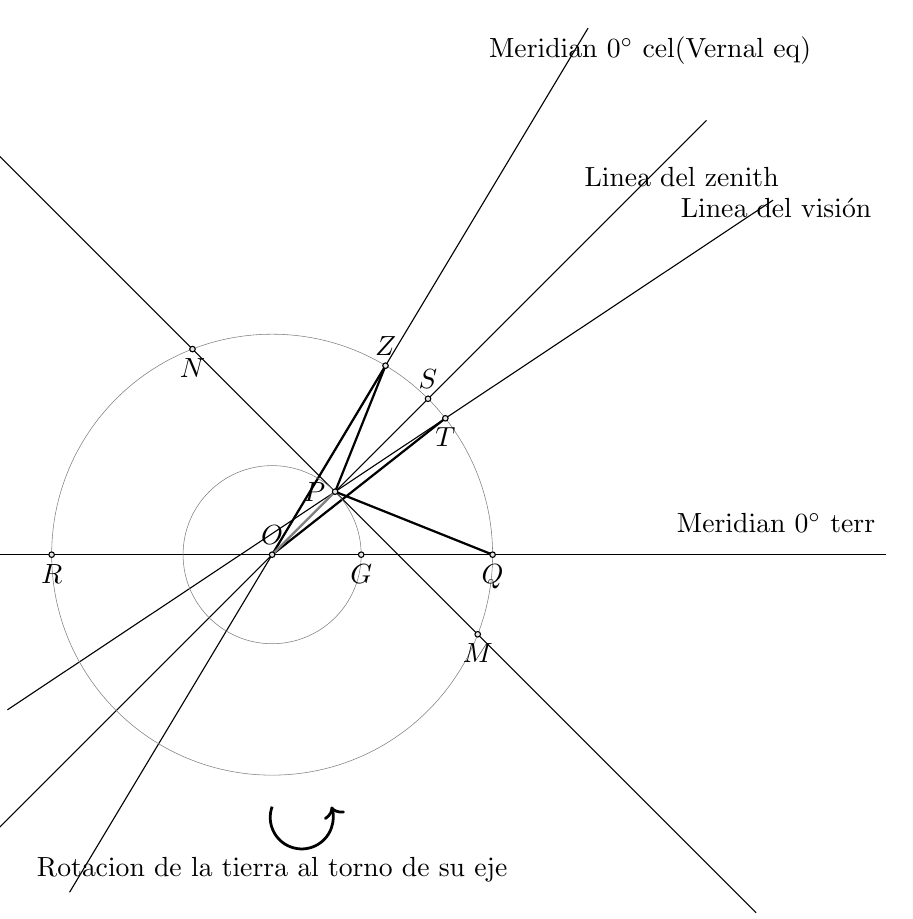
\begin{tikzpicture}[scale=.8]

% definitions
\tkzDefPoint(0,0){O}
\tkzDefPoint(1,1){P}
\tkzDefPoint(3.5,0){Q}
\tkzDefPoint(-3.5,0){R}
\tkzDefPoint(2.75,2.165){T}
\tkzDefPoint(1.8, 3){Z}
\node at (8,0.5){Meridian 0$^\circ$ terr} ; 
\node at (6,8){Meridian 0$^\circ$ cel(Vernal eq)} ; 
\node at (6.5,6){Linea del zenith} ; 
\node at (8,5.5){Linea del visión} ; 

\tkzDefPointWith[orthogonal](P,O) \tkzGetPoint{P1} % find a point P1 orthogonal to PO
\tkzInterLC(P,P1)(O,Q) \tkzGetPoints{M}{N} % find intersections of a line passing through A and Q with the large circle 
\tkzInterLC(O,P)(O,Q) \tkzGetPoints{P4}{S} % find intersections of a line passing through A and Q with the large circle 
\tkzInterLC(Q,R)(O,P) \tkzGetPoints{G}{P5} % find intersections of a line passing through A and Q with the large circle 
\draw [shorten >= -5cm, shorten <=-5cm] (P4)--(S);
\draw [shorten >= -5cm, shorten <=-5cm] (O)--(Q) ;
\draw [shorten >= -5cm, shorten <=-5cm] (O)--(Z) ;
\draw [shorten >= -5cm, shorten <=-5cm] (P)--(T) ;
\draw [shorten >= -5cm, shorten <=-5cm] (M)--(N) ;
%\tkzMarkAngle[label=lat, size=1](Q,O,P)

%\tkzDrawSegments[thick](O,T)
%\tkzDrawSegments[thick](T,Q)
\tkzDrawSegments[thick](P,Q)
\tkzDrawSegments[thick](P,Z)
\tkzDrawSegments[thick](O,Z)
\tkzDrawSegments[thick](O,T)
%\tkzMarkAngle[](Q,O,T)
%\tkzMarkAngle[label=dec, size=1](Q,P,T)
%\tkzMarkAngle[label=zd, size=1](P4,P,T)
% drawing
\tkzDrawCircle(O,P)
\tkzDrawCircle(O,Q)
\draw [->,line width=1pt] (0,-4) arc[x radius=0.5cm, y radius =.5cm, start angle=-200, end angle=20];
\node at (0,-5){Rotacion de la tierra al torno de su eje} ; 
\tkzDrawSegments[thick,gray](O,P)
\tkzDrawPoints(O,P,Q,T,M,S,N,Z,R,G)

% labels
\tkzLabelPoints(Q,T,M,N,R,G)
\tkzLabelPoints[left](P)
\tkzLabelPoints[above](O,Z,S)
\end{tikzpicture}

\vspace{5cm}
\begin{itemize}
\item Z vernal equinox
\item G punto en la tierra en el meridiano 0
\item $\angle{ZOQ}$ UniversalTime
\item $\angle{ZPT} \approx \angle{ZOT}$ RightAscension
\item $\angle{ZPS} \approx \angle{ZOS}$ SiderealTime
\item $\angle{SPT} \approx \angle{SOT}$ object hour
\item (ST = RA + h), cuando el objeto a observar está justo arriba(h=0) ST = RA
\item $\angle{QOP}$ longitud
\end{itemize}


\begin{description}
\item Cuando Sidereal Time es aprox 0 UT representa la longitud
\item longitud 22:21:45(hours) = -24:34:45(degrees)    

\end{description}

\subsection*{Instrumento}
\url{http://www.ing.iac.es/astronomy/instruments/wfc/index.html}

\subsection*{Noise}
En los headers de las imagenes(y en la especificacion de la pagina web para exposisiones largas(48 sec) - exposiciones cortas(29 sec)):
\begin{description}
\item GAIN    =                   2.  /  gain, electrons per adu (1.26 - 2.5)
\item RDNOISE =                  5.4  /  read noise, electrons (4.6 - 9)
\end{description}

En la pagina web:
\begin{description}
\item Noise(ADU) (3.7 - 3.6)
\item Bias (2030 - 1830)
\end{description}

\subsection*{Field of view and detector size}
En la pagina web:
\begin{description}
\item Field of View 34x34arcmin
\item Pixel scale 0.333 arcsec / pixel
\item pixel size = 13.5 microns
\end{description}


\begin{description}
\item Numero de pixeles del detector = FOV / pixel scale = 6126 x 6126, diferente al numero de pixeles por filas y columnas del header de las imagenes fits 
\item tamaño del detector = num pixeles * pixel size = 82.7 mm
\end{description}



\subsection*{Reducción de las imagenes}
\begin{itemize}
\item eliminar pixeles malos: ccdmask
De fornma adicional quiero aplicar otro mask y quiero definir columnas 660 y 678 como columnas malas(para corregir por ejemplo img 65) y uso un fichero mask de forma:
\begin{verbatim}
cols (660,660) || cols (678,678) ? 1 : 0
\end{verbatim}
pero sale un error: "segmentation violation". Pero funciona con un fichero mask definido:
\begin{verbatim}
circle (220., 220., 50.) && circle (240., 220., 50.) ? 1 : 0
\end{verbatim}





\end{itemize}

\end{document}
